\documentclass{article} 
\usepackage{tikz} 
\usepackage{graphicx}
\usepackage{caption}
\begin{document} 

\textbf{Exercitiul 3. (a1) }

La fiecare pas al algoritmului, functia $Search()$ alege arcul $e = ij$ cu costul minim $u_i + a_{ij}$, unde $i \in S,j \notin S$. Daca adaugam un nod la $S$, cu siguranta stim si costul lui minim $u_i$. Cum algoritmul alege doar nodul cu costul \textbf{minim} la fiecare iteratie (\textbf{while}), nodurile sunt adaugate la $S$ crescator in functie de cost.

\begin{figure}[h!]
  \centering
  \renewcommand{\thefigure}{}
  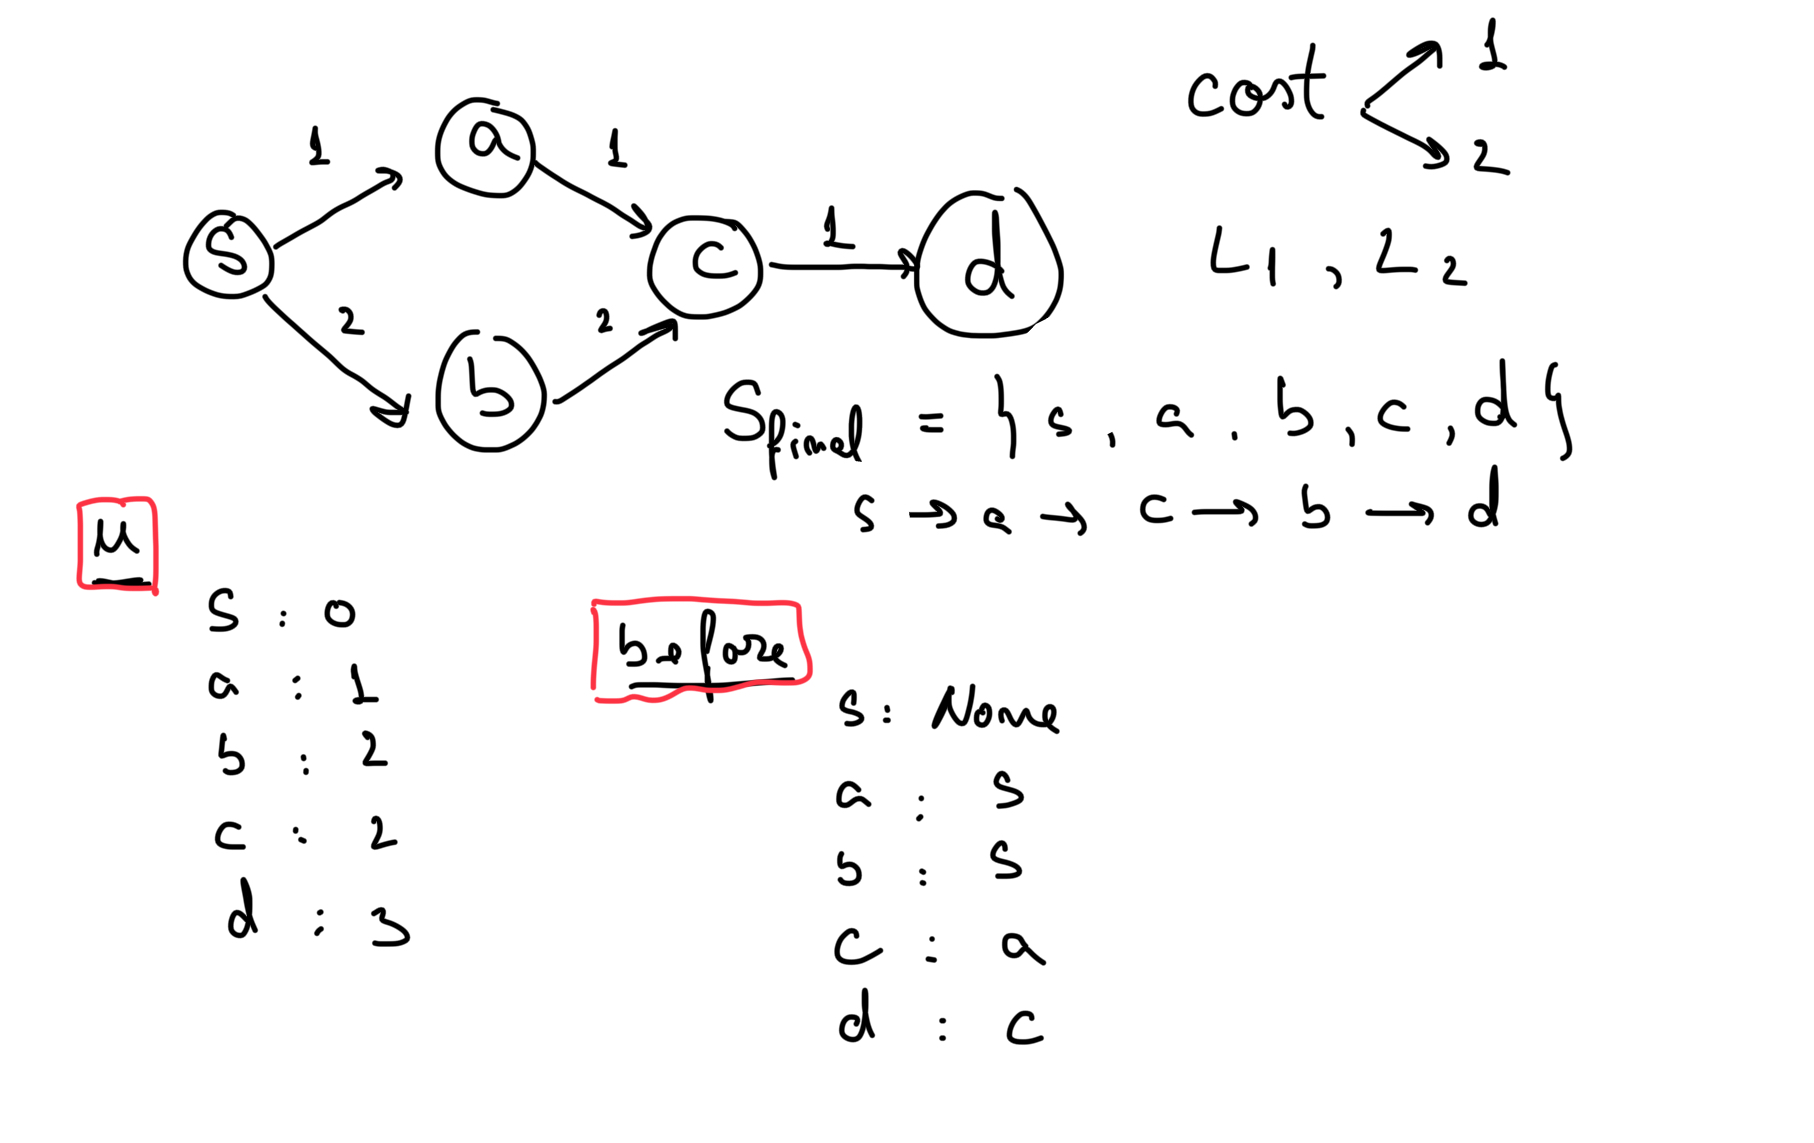
\includegraphics[width=0.7\textwidth]{example_digraf.jpg}
  \caption{Costurile minime si predecesorii obtinuti dupa executia algoritmului.}
  \label{fig:my_image}
\end{figure}

In exemplul de mai sus, ordinea in care adaugam la S este urmatoarea : $[a]$, $[a, c]$, $[a, c, b]$, ... $Search()$ cauta nodul minim dintre $(s, b)$ si $(a, c)$ si alege $(a, c)$ pentru ca are costul minim. Astfel $c$ va fi adaugat la $S$ inaintea lui $b$.

Asadar, nodurile sunt adaugate la $S$ in ordine crescatoare a costurilor minime.

\textbf{Exercitiul 3. (a2) }


\end{document}

